% The packages used here are just a sample. You may need others, and may not need some of these. It doesn't hurt to leave them in, unless they start to conflict with other packages you've added. Chapter 2 has example code for equations, figures, tables, citations, abbreviations, etc. If there are sections labeled 'optional' that you don't want, just comment them out. -jg

\documentclass[reqno,12pt,oneside]{report} % right-side equation numbering, 12 point font, print one-sided 
%\documentclass[reqno,12pt,twoside,openright]{report} % right-side equation numbering, 12 point font, print two-sided, Chapters start on odd pages. Rackham only accepts one-sided, so this is for personal printings.

\usepackage{rac}         % Use Rackham thesis style file
\usepackage{aas_macros}  % To allow the reading of ADS journal references in the bibliography
\usepackage[intlimits]{amsmath} % Puts the limits of integrals on top and bottom
\usepackage{amsxtra}     % Use various AMS packages
\usepackage{amsthm}
\usepackage{amssymb}
\usepackage{amsfonts}
\usepackage{graphicx}    % Add some packages for figures. Read epslatex.pdf on ctan.tug.org
\usepackage{rotating}
\usepackage{color}
\usepackage{epsfig}
\usepackage{subfigure}   % To make subfigures. Read subfigure.pdf on ctan.tug.org
\usepackage{verbatim}
\usepackage{natbib}      % Allows you to use BibTeX
\usepackage[printonlyused]{acronym} % For the List of Abbreviations. Read acronym.pdf on ctan.tug.org
\usepackage{setspace}    % Allows you to specify the line spacing
\doublespacing           % \onehalfspacing for 1.5 spacing, \doublespacing for 2.0 spacing.
\newcommand{\sun}{\ensuremath{\odot}} % sun symbol is \sun
%%%%%%%%%%%%%%%%%%%%%%%%%%%%%%%%%%%%%%%%%%%%%%%%%%%%%%%%%%%%%%%%%%%%%%%%%%%%%%%

% Various theorem environments. All of the following have the same numbering
% system as theorem.

\theoremstyle{plain}
\newtheorem{theorem}{Theorem}
\newtheorem{prop}[theorem]{Proposition}
\newtheorem{corollary}[theorem]{Corollary}
\newtheorem{lemma}[theorem]{Lemma}
\newtheorem{question}[theorem]{Question}
\newtheorem{conjecture}[theorem]{Conjecture}
\newtheorem{assumption}[theorem]{Assumption}

\theoremstyle{definition}
\newtheorem{definition}[theorem]{Definition}
\newtheorem{notation}[theorem]{Notation}
\newtheorem{condition}[theorem]{Condition}
\newtheorem{example}[theorem]{Example}
\newtheorem{introduction}[theorem]{Introduction}

\theoremstyle{remark}
\newtheorem{remark}[theorem]{Remark}
%%%%%%%%%%%%%%%%%%%%%%%%%%%%%%%%%%%%%%%%%%%%%%%%%%%%%%%%%%%%%%%%%%%%%%%%%%%%%%%

\numberwithin{theorem}{chapter}     % Numbers theorems "x.y" where x
                                    % is the section number, y is the
                                    % theorem number

%\renewcommand{\thetheorem}{\arabic{chapter}.\arabic{theorem}}

%\makeatletter                      % This sequence of commands will
%\let\c@equation\c@theorem          % incorporate equation numbering
%\makeatother                       % into the theorem numbering scheme

%\renewcommand{\theenumi}{(\roman{enumi})}

%%%%%%%%%%%%%%%%%%%%%%%%%%%%%%%%%%%%%%%%%%%%%%%%%%%%%%%%%%%%%%%%%%%%%%%%%%%%%%

% If printing two-sided, this makes sure that any blank page at the 
% end of a chapter will not have a page number. 
\makeatletter
\def\cleardoublepage{\clearpage\if@twoside \ifodd\c@page\else
\hbox{}
\thispagestyle{empty}
\newpage
\if@twocolumn\hbox{}\newpage\fi\fi\fi}
\makeatother 

%%%%%%%%%%%%%%%%%%%%%%%%%%%%%%%%%%%%%%%%%%%%%%%%%%%%%%%%%%%%%%%%%%%%%%%%%%%%%%

%This command creates a box marked ``To Do'' around text.
%To use type \todo{  insert text here  }.

\newcommand{\todo}[1]{\vspace{5 mm}\par \noindent
\marginpar{\textsc{To Do}}
\framebox{\begin{minipage}[c]{0.95 \textwidth}
\tt\begin{center} #1 \end{center}\end{minipage}}\vspace{5 mm}\par}

%%%%%%%%%%%%%%%%%%%%%%%%%%%%%%%%%%%%%%%%%%%%%%%%%%%%%%%%%%%%%%%%%%%%%%%%%%%%%%%
\begin{document}

\bibliographystyle{agu04}    % Set the bibliography style. agu04, plain, alpha, etc.

% Title page as required by Rackham dissertation guidelines
\titlepage{The Title of Your Dissertation}{Your Name}{Doctor of Philosophy}
{Atmospheric and Space Sciences}{2008}
{Professor Albert Einstein, Chair\\
 Professor Werner Heisenberg\\
 Associate Professor Hermann von Helmholtz\\
 Associate Professor Edwin Hubble\\
 Assistant Professor John von Neumann}

% Begin the front matter as required by Rackham dissertation guidelines
\initializefrontsections

% Optional Frontispiece
\frontispiece{
\includegraphics[width=6in]{Intro/Happy} Find a cool picture to go here.}

% Optional, but recommended, Copyright page
\copyrightpage{Your Name}

% Page numbering. If you don't include a frontispiece or copyright page, you'll need to change this for two-sided printing.
\makeatletter
\if@twoside \setcounter{page}{4} \else \setcounter{page}{1} \fi
\makeatother
 
% Optional Dedication page
\dedicationpage{For all the people}

% Optional Acknowledgements page
\startacknowledgementspage
Thanks to the people who made this dissertation possible, especially those who put together a nice \LaTeX\, template for me to use.
\label{Acknowledgements}

% Optional Preface page
%\startprefacepage
%\input{Preface}
%\label{Preface}

% Table of contents, list of figures, etc.
\tableofcontents     % Required
\listoffigures       % Required if there is more than one figure
%\listoftables        % Required if there is more than one table
%\listofmaps          % Required if there is more than one map
%\listofappendices    % Required if there is more than one appendix
\listofabbreviations % Optional. Abbreviations should be stored in a file named abbr.tex

% Optional in-dissertation Abstract Page
\startabstractpage
{The Title of Your Dissertation}{Your Name}{Chair: Albert Einstein}
This template conforms to University of Michigan abstract and dissertation format guidelines as of September 2008. It is an update to a template that has been floating around among grad students here for about 20 years. The main components are the thesis.tex file and the rac.sty file, the latter of which should not need any modification. If BibTeX is used (and for a dissertation, it should be), then References.bib is also needed. If a list of acronyms is desired, make all additions in abbr.tex and read acronym.pdf on ctan.org for details on how to call them in the text. Other files in this template that may be helpful, but don't necessarily need to be used include a style file that formats your bibliography in AGU format (agu04.bst) and a style file that allows you to use abbreviations for journal names (aas\_macros.sty) when typing out the bibliography. This will be necessary if you grab BibTeX information from places like the NASA ADS, which sometimes uses journal name abbreviations. It is useful to separate chapters into their own subfolders, with each folder containing the chapter's .tex file as well as all associated figures. For the figures, just call the name of the file, without the suffix (i.e., includegraphics\{Chap5/LabSetup\}) and the graphicx package will figure out what type of file it is. To compile to pdf, some format other than .eps must be used with the figures. To compile to ps, the figures need to be in ps or eps. If using \LaTeX\, in a Windows environment, there are several different editors and programs that can be used. One set that is known to work well is the following, which can each be found with a simple web search and which should be installed in this order: a Perl distribution such as ActivePerl, a \TeX\, distribution such as MikTex, a \LaTeX\, editor such as TeXnicCenter, a postscript interpreter like Ghostscript, and a postscript viewer like GSView. I included a few pages of sample code in chapter 2 to help you get started, including code for writing equations, citations, abbreviations, tables, and calling graphics. Always be sure to compile your thesis.tex file a couple of times to get the references and page numbering updated. Good luck. -jg
\label{Abstract}

\startthechapters 
% The individual files for each of the chapters are put here.
% Save each chapter of your thesis to a seperate tex file
% and then use the \input command to include this file in your
% thesis.  For instance you can save a file to "intro.tex" and 
% then type \input{intro}. 

 \chapter{Introduction}
 \label{chap:Intro}
 The weather in space can have substantial effects on everything within the Sun's influence, including Earth. Most of the effects of space weather are mitigated by Earth's atmosphere and magnetic field, which form a barrier that much of the plasma in space cannot penetrate. Spacecraft and astronauts, however, risk exposure to potentially harmful radiation. Space weather can directly affect Earth's atmosphere, such as near Earth's poles where the magnetic field is shaped in such a way that the solar wind can interact with the upper atmosphere and create the aurora. Space weather can be dangerous, as storms from the Sun damage spacecraft and cause power outages on Earth. To protect astronauts and spacecraft from harm, an understanding of the fundamental physics behind space weather is vital. There are many unknown pieces to the puzzle, but through research and experimentation the picture is slowly being pieced together. As mankind looks toward further exploration of the Moon and the planets, the ability to forecast and protect humans from the effects of space weather become even more important.

This research examines new techniques and tools that can be used to study crucial pieces of the space weather puzzle. The emphasis is on ions found in the space environment: the solar wind (keV), pickup ions (10--100 keV), and energetic particles (100 keV--GeV). Each of these particle populations is created by a specific set of processes, described briefly in Chapter~\ref{chap:Particles}, and all have trajectories through space that are closely related to the magnetic field of the Sun and the heliosphere. Within the Alfv\'{e}n radius (10--20 R$_\sun$), where the kinetic energy of the solar wind is weaker than the energy density of the Sun's magnetic field, the solar wind is guided by the field's shape and corotates with the Sun. Beyond this radial distance, the electrically charged and highly conductive solar wind controls and shapes the magnetic field, drawing it radially outward into the heliosphere. Energetic particles travel along the lines of magnetic flux that extend from the solar surface to the outermost reaches of the solar system. To a large degree, if the shape and path of the Sun's magnetic field can be accurately mapped, the trajectories of these particles could be inferred. However, such mapping techniques have been elusive, or inaccessible to the broad community.


 \chapter{Particle Transport and Acceleration}
 \label{chap:Particles}
 \section{Introduction}
\label{Transport Intro}
For reference, some common equations and brief overviews of the three categories of particles will be given in this chapter. The Maxwell equations \eqref{Gauss}--\!\,\eqref{Ampere}, the continuity equation for charge density and current density \eqref{continuity}, the Lorentz force equation \eqref{Lorentz}, Newton's second law of motion \eqref{Newton2}, and the \ac{MHD} approximation of Ohm's Law \eqref{Ohm} are each useful for basic plasma physics. Thorough derivations for these and related equations can be found in several textbooks, including \citet{gombosi98} and \citet{jackson99}.

\begin{subequations}
 \begin{align}
  \nabla\cdot\mathbf{E}&=\frac{\rho_e}{\epsilon_0}&\quad\text{Gauss's Law}
  \label{Gauss}\\
  \nabla\times\mathbf{E}&=-\frac{\partial\mathbf{B}}{\partial t}&\quad\text{Faraday's law of induction}
  \label{Faraday}\\
  \nabla\cdot\mathbf{B}&=0&\quad\text{Gauss's law for magnetism}
  \label{Gauss m}\\
  \nabla\times\mathbf{B}&=\mu_0\mathbf{J}+\mu_0\epsilon_0\frac{\partial\mathbf{E}}{\partial t}&\quad\text{Amp\`{e}re's law}
  \label{Ampere}
 \end{align}
\end{subequations}
\begin{align}
 \nabla\cdot\mathbf{J}&=-\frac{\partial\rho_e}{\partial t}&\quad\text{continuity equation}
 \label{continuity}\\
 \mathbf{F}&=q\left(\mathbf{E}+\mathbf{v}\times\mathbf{B}\right)\quad\text{(N)}&\quad\text{Lorentz force}
 \label{Lorentz}\\
 \mathbf{F}&=m\mathbf{a}\quad\text{(N)}&\quad\text{Newton's 2nd law of motion}
 \label{Newton2}\\
 \mathbf{J}&=\sigma\left(\mathbf{E+v\times B}\right)\quad\text{(A m$^{-2}$)}&\quad\text{Ohm's law}
 \label{Ohm}
\end{align}

In these equations, $\epsilon_0$ is the electric constant (also called the permittivity of free space), $\mu_0$ is the magnetic constant (also called the permeability of free space), $\sigma$ is the electrical conductivity, treated here as a constant, $q$ is the charge, $\rho_e$ is the charge density, $m$ is the mass, $\mathbf{J}$ is the electric current density, and $\mathbf{E}$ and $\mathbf{B}$ are the electric and magnetic fields. $\mathbf{F}$, $\mathbf{v}$, and $\mathbf{a}$ represent force, velocity, and acceleration. 

In \ac{MHD}, the fields are induced by plasma motion, so the fields vary on the same time and length scales as the plasma variables. If high frequency variations in the electric field are not included, and only the non-relativistic regime is considered, the displacement current in Amp\`{e}re's law can be neglected, leading to Equation~\ref{AmpereMHD}.
\begin{align}
 \nabla\times\mathbf{B}&=\mu_0\mathbf{J}&&\quad\text{MHD Amp\`{e}re's law}
 \label{AmpereMHD}
\end{align}
\indent By substituting Equation~\ref{Faraday} and the curl of Equation~\ref{AmpereMHD} into the curl of Equation~\ref{Ohm}, $\mathbf{E}$ and $\mathbf{J}$ can be eliminated to derive the magnetic induction equation \eqref{MHDinduction}. The first term on the right describes the resistive diffusion of the magnetic field in the plasma while the second term describes the convection of the magnetic field by the plasma.
\begin{align}
 \frac{\partial\mathbf{B}}{\partial t}=\frac{1}{\sigma\mu_0}\nabla^2\mathbf{B}+\nabla\times\left(\mathbf{v}\times\mathbf{B}\right)&&\quad\text{magnetic induction equation}
 \label{MHDinduction}
\end{align}

Since Equation~\ref{Gauss m} states that the divergence of the magnetic field vector $\mathbf{B}$ is zero, $\mathbf{B}$ can be written in terms of a vector potential $\mathbf{A}$:
\begin{align}
 \mathbf{B}=\nabla\times\mathbf{A}\quad\text{(T)}.
 \label{B field}
\end{align}

By substituting Equation~\ref{B field} into Equation~\ref{Faraday}, Faraday's law of induction can be written as a quantity with a vanishing curl. Such a quantity can be rewritten as the gradient of a scalar function, the scalar potential $\Phi$, leading to an equation for $\mathbf{E}$ in terms of the potentials $\mathbf{A}$ and $\Phi$:
\begin{align}
 \mathbf{E}=-\nabla\Phi-\frac{\partial\mathbf{A}}{\partial t}\quad\text{(V m$^{-1}$)}.
 \label{E field}
\end{align}

For electrostatics, all derivatives with respect to time are zero. In this case, the divergence of Equation~\ref{E field} combined with Equation~\ref{Gauss} will give the Poisson equation, or in the absence of charges, the Laplace equation:
\begin{align}
 \nabla^2\Phi &= -\frac{\rho_e}{\epsilon_0},&\quad\text{Poisson's equation}
 \label{Poisson}\\
 \nabla^2\Phi &= 0.&\quad\text{Laplace's equation}
 \label{Laplace}
\end{align}

Due to the historical precedent of the symbols used in these and other common equations, a symbol may have different meanings depending on the equation in which it is used (i.e., `E' can represent `electric field' or `energy'). Even though the meaning of the symbol can usually be discerned from the context of the equation, an attempt has been made to use distinct symbols throughout this dissertation, or use subscripts to clarify a symbol's meaning when necessary. In the specific case of `E', the bold font $\mathbf{E}$ is used to represent the electric field vector and $\left|\mathbf{E}\right|$  to represent the magnitude of the electric field. The plain font E is always used here to represent energy.

Particle transport and acceleration are important topics of research in heliophysics. An understanding of the composition and nature of the gas and plasma found in space is vital to the forecasting of space weather. This research focuses on ways to investigate three categories of particles: the solar wind (\S~\ref{Solar Wind}), pickup ions, and energetic particles, as shown in Figure~\ref{fig:H_Distribution}. The following is intended to provide sufficient background for the scope of this dissertation research.
\begin{figure}
  \centering
  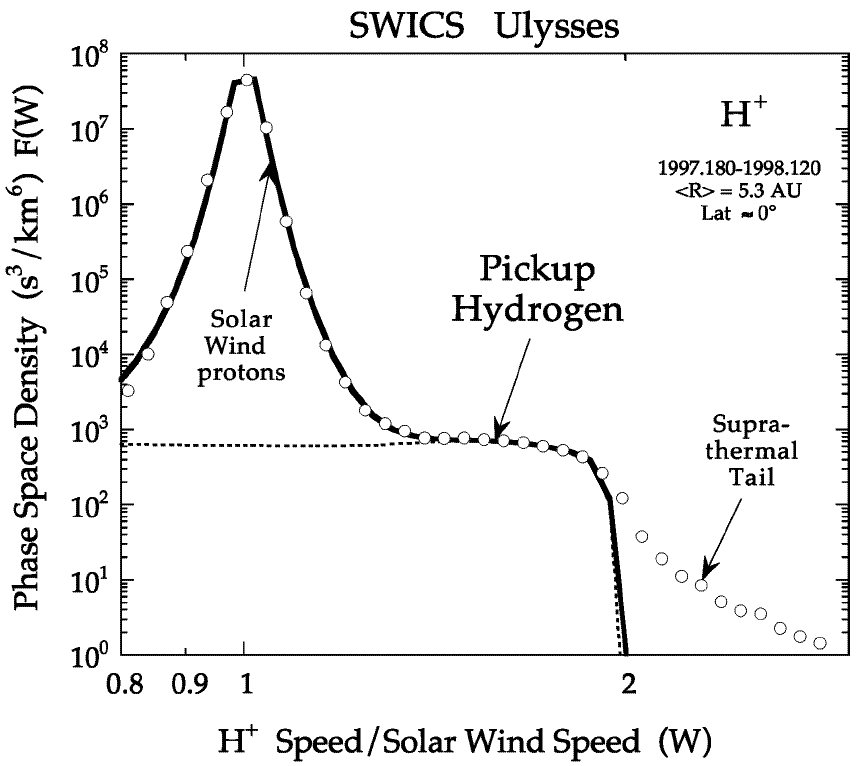
\includegraphics[width=.65\textwidth]{Chap2/H_Distribution}
  \caption[Example of proton distributions for the quiet solar wind near 5 AU.]{Example of proton distributions for the quiet solar wind near 5 AU. Shown are the bulk distribution of the solar wind, the interstellar pickup ions that drop off at twice the solar wind speed, and the high-energy protons that make up the suprathermal tail. Figure from \citet{gloeckler01b}.}
  \label{fig:H_Distribution}
\end{figure}

\section{The Solar Wind}
\label{Solar Wind}

\subsection{Current Knowledge}
\label{SW Current Knowledge}
While he was not the first to postulate its existence, the physics of the solar wind was first explained by Eugene Parker in 1958 \citep{parker58}. Beginning with subsonic speeds close to the Sun, plasma accelerates away from the solar surface and reaches supersonic speeds in the corona. It continues to expand in a radial direction outward until it interacts with the material in interstellar space at the edge of the heliosphere, the Sun's sphere of influence. The wind draws the solar magnetic field along with it, creating spiral-shaped field lines as the Sun rotates \citep{parker59}. Mankind's understanding of the processes that govern the solar wind has increased as spacecraft have taken in situ measurements, but there are still some properties that remain unexplained, such as the precise origin of certain types of wind, as discussed below.

The solar wind travels a distance of one \ac{AU} before reaching Earth's orbit, where most of the current measurements have been taken (Table~\ref{tab:solar wind}). It is generally divided into two components, commonly referred to as the ``fast'' and ``slow'' solar wind. Originally, these terms were used to differentiate the wind by the speed with which it traveled, but more recent studies have shown that the two types of wind are more efficiently distinguished by their charge state composition (e.g., O$^{7+}$/O$^{6+}$) since the plasma can change speeds as it flows through space \citep{geiss95b, gloeckler03a}. Rather than the terms ``fast'' and ``slow'', more appropriate labels are descriptive of the wind's origin: ``coronal hole'' and ``streamer'' wind. These two types of wind are generated by different processes and have different compositions, temperatures, speeds, and origins.
\begin{table}[htbp]
	\centering
		\begin{tabular}{l|c|c}
		                                                               & Coronal Hole Wind & Streamer Wind     \\ \hline
      bulk speed \footnotesize{$\left(\text{km s}^{-1}\right)$}    & 750               & 400               \\ \hline
      thermal speed \footnotesize{$\left(\text{km s}^{-1}\right)$} & 32                & 35                \\ \hline
      H$^+$ density \footnotesize{$\left(\text{cm}^{-3}\right)$}   & 2.5               & 8.7               \\ \hline
      frozen-in temperature \footnotesize{$\left(\text{K}\right)$} & 8 x 10$^5$        & 1.4--1.6 x 10$^6$ \\ \hline

		\end{tabular}
	\caption[Average characteristics of the solar wind at 1 AU.]{Average characteristics of the solar wind at 1 AU. The temperature is derived from the freeze-in temperature of C$^{6+}$/C$^{5+}$, which freezes in near the solar wind source altitude. Data compiled from \citet{vonsteiger95, gloeckler98a, ipavich98, mccomas00, feldman05}.}
	\label{tab:solar wind}
\end{table}

As solar wind ions escape from the photosphere and travel up through the corona, they experience collisions with energetic electrons that ionize them to different degrees. As they travel farther through the corona, continuously accelerating, the density of coronal electrons decreases and the particles experience fewer collisions. When the timescale for ionization or recombination becomes longer than the timescale of the solar wind to expand through a density scale height, the charge state of the ion is said to be ``frozen in,'' branding the ion with the coronal region and electron temperature of its origin \citep{hundhausen68}. The streamer wind has a distinct characteristic of being enriched in elements with a low ($\le$ 10 eV) \ac{FIP} by a factor of 3--4 over the photospheric value. The coronal hole wind does not show this density enhancement, and measurements have revealed abundances of low-\ac{FIP} elements that match ratios in the photosphere \citep{vonsteiger93}. The streamer wind also has a higher and more variable freeze-in temperature than the coronal hole wind. One explanation for this describes solar plasma trapped and heated in large coronal loops that are eventually opened by interchange reconnection, releasing the plasma \citep{gosling95, fisk98, fisk99a}.

The coronal hole wind originates in the open flux regions of the Sun, which contain low-density plasma and concentrations of magnetic flux that are all the same polarity. During solar minimum these regions are clustered around the poles of the Sun, while during solar maximum they appear at all latitudes. Plasma in open flux regions is also released from flux loops, but the high concentration of open flux increases the probability that the loops will open before they can heat and fractionate the plasma. The anti-correlation between freeze-in temperature and solar wind speed shown in Table~\ref{tab:solar wind} can be interpreted in a simplistic way as a sign of different sized loops. The long-lived loops that produce the streamer wind will expand and rise slowly into the corona, where the temperatures are hotter, before being opened \citep{fisk98, fisk01a}. The short-lived loops that yield the coronal hole wind are opened while they are still small and close to the cooler surface \citep{fisk99a, fisk03, wimmer03b}.

\startappendices
 \appendix{Two-Dimensional Crank-Nicolson Scheme for a Uniform Spherical Grid}
 \label{app:CN Scheme}
 For the diffusion process, The equation was solved using a two-dimensional implicit Crank-Nicolson scheme, which is unconditionally stable and second-order accurate in both time and space \citep{crank47}. In the conventional notation, the two-dimensional numerical scheme using central differencing can be written for a uniform Cartesian grid as 
\begin{eqnarray}
\nonumber\left(1+2\mu\right)u^{t+1}_{i,j}-\frac{\mu}{2}\left(u^{t+1}_{i+1,j}+u^{t+1}_{i-1,j}+u^{t+1}_{i,j+1}+u^{t+1}_{i,j-1}\right)\\
=\left(1-2\mu\right)u^{t}_{i,j}+\frac{\mu}{2}\left(u^{t}_{i+1,j}+u^{t}_{i-1,j}+u^{t}_{i,j+1}+u^{t}_{i,j-1}\right),
\end{eqnarray}

\noindent where $u^{t}_{i,j}$ is the value of the parameter undergoing the diffusion ($B_{r}$ in this case) at position $(i, j)$ at time \textit{t}. The von Neumann number on a uniform grid is $\mu=\xi{\Delta}t/\left({\Delta}x\right)^{2}$, where the size of the grid square is $\Delta x$ on each side, and the diffusion coefficient $\xi$ describes the speed at which the mathematical diffusion takes place. When deriving the two-dimensional Crank-Nicolson scheme in spherical coordinates, the von Neumann number is written as $\mu=\xi{\Delta}t/\left(r\Delta\theta\right)^{2}$, where $\Delta\theta=\Delta\phi$, and the cosine is replaced by the central difference of the sine to remain consistent with the discrete nature of the other terms. Care must be taken at the poles, where the central differencing is replaced by forward or backward differencing. To keep second-order accuracy with forward or backward differencing, the series must be carried out to higher-order terms in the derivation. The two-dimensional numerical scheme using central differencing can be written for a uniform spherical grid as
\begin{multline}
\left(1+\mu+\frac{\mu}{\sin^{2}\theta_{i,j}}\right)u^{t+1}_{i,j}-\frac{\mu}{2}\left[1+\frac{\left(\sin\theta_{i+1,j}-\sin\theta_{i-1,j}\right)}{4\sin\theta_{i,j}}\right]u^{t+1}_{i+1,j}\\
 -\frac{\mu}{2}\left[1-\frac{\left(\sin\theta_{i+1,j}-\sin\theta_{i-1,j}\right)}{4\sin\theta_{i,j}}\right]u^{t+1}_{i-1,j}-\frac{\mu}{2}\frac{1}{\sin^{2}\theta_{i,j}}u^{t+1}_{i,j+1}-\frac{\mu}{2}\frac{1}{\sin^{2}\theta_{i,j}}u^{t+1}_{i,j-1}\\
 =\left(1-\mu-\frac{\mu}{\sin^{2}\theta_{i,j}}\right)u^{t+1}_{i,j}+\frac{\mu}{2}\left[1+\frac{\left(\sin\theta_{i+1,j}-\sin\theta_{i-1,j}\right)}{4\sin\theta_{i,j}}\right]u^{t+1}_{i+1,j}\\
 +\frac{\mu}{2}\left[1-\frac{\left(\sin\theta_{i+1,j}-\sin\theta_{i-1,j}\right)}{4\sin\theta_{i,j}}\right]u^{t+1}_{i-1,j}+\frac{\mu}{2}\frac{1}{\sin^{2}\theta_{i,j}}u^{t+1}_{i,j+1}+\frac{\mu}{2}\frac{1}{\sin^{2}\theta_{i,j}}u^{t+1}_{i,j-1}.
 \label{CN Spherical}
\end{multline}

Although it is unconditionally stable, a marching scheme such as this will depend on the value of $\mu$ for its accuracy. A lower choice of $\mu$ will lead to a more accurate solution at the expense of computational resources (i.e., a smaller time step ${\Delta}t$), while a higher value of $\mu$ will arrive at a solution more rapidly but with less accuracy (a larger time step). In this model, the value of the coefficient $\xi$ describes the speed of the mathematical relaxation and, since it does not describe a physical process, can be chosen arbitrarily. Thus the only restriction for this scheme will lie in keeping $\mu$ small for accuracy and assigning either $\xi$ or ${\Delta}t$. It can be seen that when $\mu$ is held constant, any choice for either $\xi$ or ${\Delta}t$ will lead to the same solution. A value of $\mu=1/4$ was chosen, with an arbitrary time step of ${\Delta}t=0.1$ s, and studied several different grid resolutions, with a grid size of 2.5$^\circ$ x 2.5$^\circ$ (72 x 144 grid spaces) on a uniform spherical grid used for the comparisons in this paper. The relaxation was allowed to continue on a sphere of $r=R_{\sun}$ until the difference in magnetic field magnitude between any cell and its neighbor was of order $10^{-1}{\mu}T$.
 
\startbibliography
 \begin{singlespace} % Bibliography must be single spaced
  \bibliography{References}   % Use the BibTeX file ``References.bib''.
 \end{singlespace}

% An external Abstract that can be printed at the end of the document, 
% for separate submission to Rackham. Comment it out when not needed. - jg
%\startextabstractpage
%{The Title of Your Dissertation}{Your Name}{Chair: Albert Einstein}
%This template conforms to University of Michigan abstract and dissertation format guidelines as of September 2008. It is an update to a template that has been floating around among grad students here for about 20 years. The main components are the thesis.tex file and the rac.sty file, the latter of which should not need any modification. If BibTeX is used (and for a dissertation, it should be), then References.bib is also needed. If a list of acronyms is desired, make all additions in abbr.tex and read acronym.pdf on ctan.org for details on how to call them in the text. Other files in this template that may be helpful, but don't necessarily need to be used include a style file that formats your bibliography in AGU format (agu04.bst) and a style file that allows you to use abbreviations for journal names (aas\_macros.sty) when typing out the bibliography. This will be necessary if you grab BibTeX information from places like the NASA ADS, which sometimes uses journal name abbreviations. It is useful to separate chapters into their own subfolders, with each folder containing the chapter's .tex file as well as all associated figures. For the figures, just call the name of the file, without the suffix (i.e., includegraphics\{Chap5/LabSetup\}) and the graphicx package will figure out what type of file it is. To compile to pdf, some format other than .eps must be used with the figures. To compile to ps, the figures need to be in ps or eps. If using \LaTeX\, in a Windows environment, there are several different editors and programs that can be used. One set that is known to work well is the following, which can each be found with a simple web search and which should be installed in this order: a Perl distribution such as ActivePerl, a \TeX\, distribution such as MikTex, a \LaTeX\, editor such as TeXnicCenter, a postscript interpreter like Ghostscript, and a postscript viewer like GSView. I included a few pages of sample code in chapter 2 to help you get started, including code for writing equations, citations, abbreviations, tables, and calling graphics. Always be sure to compile your thesis.tex file a couple of times to get the references and page numbering updated. Good luck. -jg
%\label{ExtAbstract}

\end{document}